% Устранение самопересечений
\subsection{Устранение самопересечений расчетной сетки}

В предыдущих разделах рассматривались ситуации, когда во время перестроения расчетной сетки возникали конфликты из-за сворачивания отдельных ячеек.
В отдельных случаях появление этих конфликтов можно предотвратить с помощью сглаживания нормалей, как это описано в разделе~\ref{sec:tong_method}.
Но наиболее серьезной проблемой, которая может возникнуть при перестроении сетки, является пересечение эволюционирующей поверхности с самой собой, которое будем называть самопересечением \cite{Freylekhman2022GeoIntersect}\label{term:mesh_self_intersect}.
Самопересечение является критическим дефектом сетки, при котором невозможно производить дальнейшие вычисления по моделированию ледообразования, поэтому самопересечения необходимо удалять.
В общем случае предотвратить самопересечение невозможно, так как в процессе ледообразования при активном нарастании льда возможно переречение одних ледяных наростов с другими ледяными наростами.
Таким образом, для адекватного моделирования процесса ледообразования необходимо уметь корректно обрабатывать самопересечения расчетной сетки, чтобы после возникновения самопересечения можно быть продолжать выполнение расчетов.

\subsubsection{Адаптация}

Все рассмотренные в разделе~\ref{sec:text_1_remesh_3d} методы перестроения поверхностей объединяет одно сходство -- они сохраняют количество элементов расчетной сетки (узлы, ребра, грани) и связи между ними.
Несмотря на некоторые специальные методы по предотвращению конфликтов между гранями сетки и методы сглаживания, после формирования новой поверхности возможно возникновение самопересечений, появление граней неправильной формы, а также неравномерное распределение граней в сетке по размеру.
Пока опустим самопересечения сетки и будем рассматривать только вопросы, касающиеся формы и размера ячеек.

\begin{figure}[ht]
\centering
\begin{tabular}{ll}
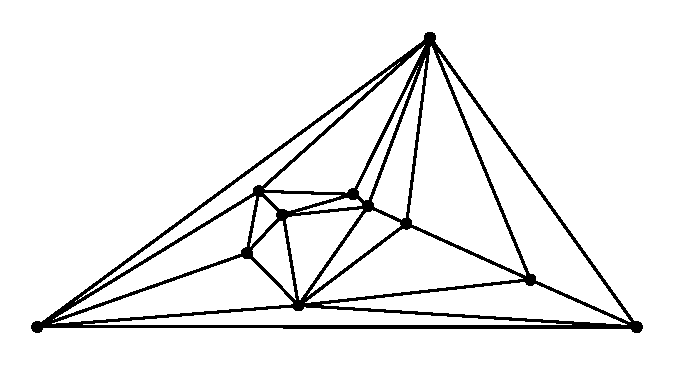
\includegraphics[width=0.35\textwidth]{./pics/text_1_int/pic_delaunay.pdf}
&
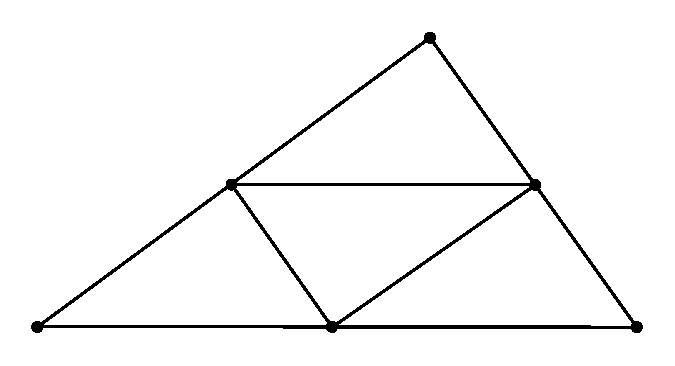
\includegraphics[width=0.35\textwidth]{./pics/text_1_int/pic_delaunay_2.pdf}
\end{tabular}
\singlespacing
\captionstyle{center}\caption{Разбиение ячейки на более мелкие треугольники.}
\label{fig:text_1_int_cut}
\end{figure}

Первая операция, которая нам потребуется -- разбиение ячейки на более мелкие.
Во всех случаях будем выполнять разбиение ячеек с помощью триангуляции Делоне, считая что для разбиения нам известен набор точек внутри разбиваемой ячейки (рис.~\ref{fig:text_1_int_cut} слева) \cite{Rivara2019Delaunay}.
Стоит отметить, что разбиение ячейки можно производить с сохранением локальной кривизны сетки, как это показано в \cite{Rakotoarivelo2019Remesh}, но для простоты будем производить разбиение исключительно в плоскости ячейки.
Если точка разбиения находится не внутри ячейки, а на ее ребре, то разбить придется также вторую инцидентную ячейку этого ребра (рассматриваются только сетки, ребра которых имеют ровно по две инцидентные ячейки, как это указано в \eqref{eqn:text_1_remesh3_arch}).
Иногда для уменьшения размера требуется просто разбить ячейку на более мелкие без задания точек разбиения.
В этом случае необходимо следить за качеством результирующих ячеек.
Для определения качества формы ячейки треугольной формы с узлами $A$, $B$, $C$ можно пользоваться простым критерием качества
\begin{equation}
Q(f) = \frac{4\sqrt{3} S_{ABC}}{|\overline{AB}|^2 + |\overline{BC}|^2 + |\overline{AC}|^2},
\end{equation}

где $Q(f) = 1$ соответствует идеальному случаю равносторонней ячейки, а $Q(f) = 0$ -- худший случай для ячеек с нулевой площадью \cite{Borouchaki2000Remesh}.
Для выполнения разбиения ячейки на более мелкие с сохранением их качества просто выполним разбиение по серединам всех ее сторон (рис.~\ref{fig:text_1_int_cut} справа).

\begin{figure}[ht]
\centering
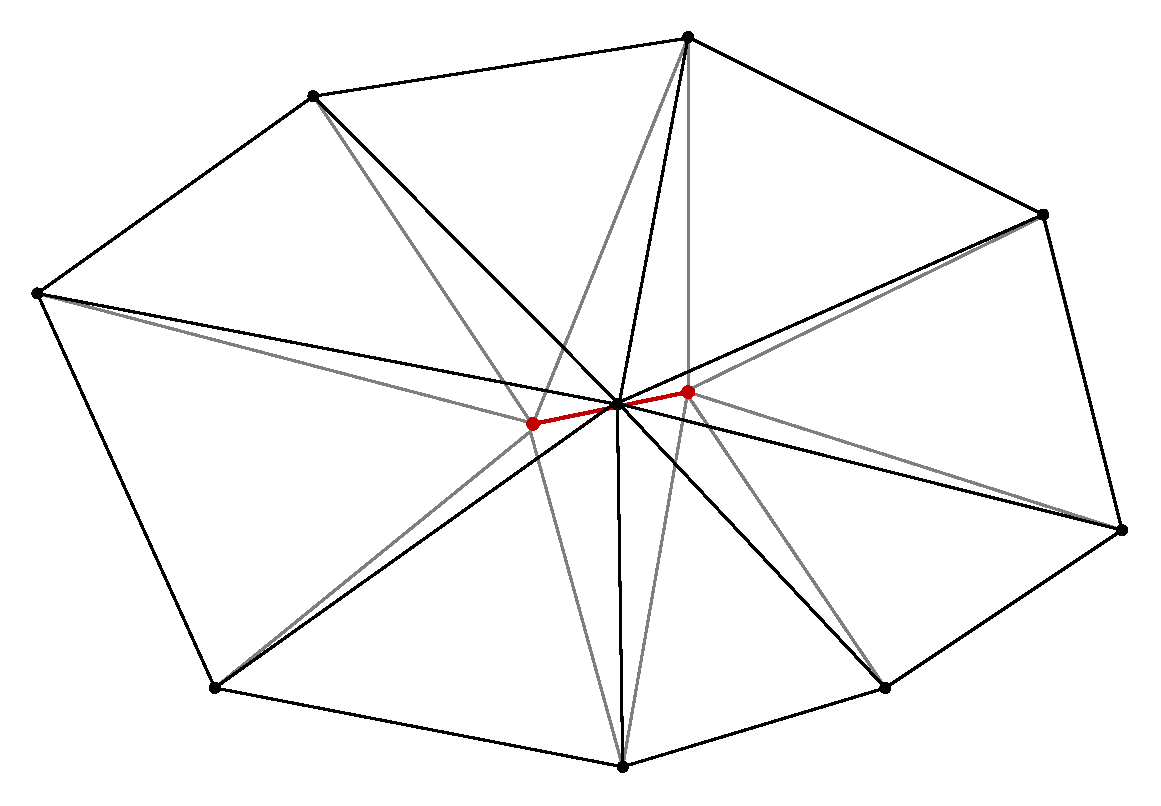
\includegraphics[width=0.4\textwidth]{pics/text_1_int/pic_reduce_edge.pdf}
\singlespacing
\captionstyle{center}\caption{Удаление короткого ребра.}\label{fig:text_1_int_reduce_edge}
\end{figure}

Вторая операция, которая необходима для адаптации сетки, связана с огрублением.
Достаточно часто во время выполнения триангуляции по множеству заданных точек могут появляться ячейки с низким показателем качества (у них могут присутствовать либо слишком острые углы, либо близкий к развернутому угол).
Если в ячейке присутствует угол, близкий к развернутому, то избавиться от него поможет разбиение по наибольшей стороне (при этом в качестве точки разбиения следует выбрать основание высоты, опущенной из противолежащего узла).
Если же в треугольнике присутствуют лишь близкие к острым углы, то значит в нем есть слишком короткая сторона, которая может быть удалена.
При удалении ребра $AB$ удаляются обе инцидентные ей грани, узлы $A$ и $B$ соединяются в единый узел $A'$, а все ребра из множества $\mathscr{E}(A) \cup \mathscr{E}(B)$ перенаправляются на узел $A'$ с учетом удаления повторных (рис.~\ref{fig:text_1_int_reduce_edge}).
Эту операцию будем называть стягиванием ребра \cite{Panchal2022Tri}.
Путем применения стягивания наиболее коротких ребер в расчетной сетке можно добиться произвольной степени огрубления.

%---------------------------------------------------------------------------------------------------

\subsubsection{Поиск пересекающихся ячеек}

Для поиска самопересечения необходимо определить, какое отношение двух ячеек сетки можно трактовать как самопересечение.
Конечно, простое наличие общих точек у двух ячеек не может служить критерием самопересечения, так как у каждой ячейки есть смежные ячейки (то есть две ячейки могут иметь как общую вершину, так и общее ребро).
Так как смежными могут быть только ячейки, имеющие общие инцидентные объекты (общую инцидентную вершину или общее инцидентное ребро), а все отношения инцидентности зафиксированы в расчетной сетке, то не представляет труда отделить пересечение ячеек по общему инцидентному объекту от самопересечения.

В любом случае для идентификации всех фактов самопересечения сетки требуется проанализировать все пары ячеек и проверить пересечение ячеек в паре (то есть проверить пересечение каждой ячейки с каждой).
Так как прямой перебор всех пар ячеек имеет квадратичную сложность по количеству ячеек в сетке, то его использование на крупных сетках невозможно.
В этом случае целесообразно выполнять поиск пар пересекающихся ячеек с помощью представления множества ячеек в виде специальной древовидной структуры, связанной с ограничением геометрических объектов прямоугольными параллелепипедами в пространстве.
Для начала определим понятие контейнера для произвольного множества точек $M$ в пространстве (будем обозначать его через $[M]$): $[M]$ -- это прямоугольный параллелепипед, являющийся декартовым произведением трех сегментов
\begin{equation}
[M] = \left[\min_{P \in M}{P_x}, \max_{P \in M}{P_x}\right]
      \times \left[\min_{P \in M}{P_y}, \max_{P \in M}{P_y}\right]
      \times \left[\min_{P \in M}{P_z}, \max_{P \in M}{P_z}\right]
\end{equation}

Контейнер можно рассматривать для произвольного множества точек.
Мы будем его использовать для ячейки расчетной сетки, а также для множества ячеек.
Так как любой треугольник является выпуклой фигурой, то $[ABC] = [\{A, B, C\}]$, то есть для построения контейнера для треугольника достаточно рассмотреть только его вершины.
При поиске пар пересекающихся ячеек будем использовать следующий факт: если два треугольника пересекаются, то пересекаются и их контейнеры: $ABC \cap A'B'C' \ne \emptyset \implies [ABC] \cap [A'B'C'] \ne \emptyset$.
А значит если не пересекаются контейнеры двух треугольников, то не пересекаются и сами треугольники: $[ABC] \cap [A'B'C'] = \emptyset \implies ABC \cap A'B'C' = \emptyset$.
В отличие от анализа пары треугольников на пересечение, проверка на пересечение двух прямоугольных параллелепипедов со сторонами, параллельными координатным осям, является простой операцией.
То есть па первом этапе будем искать такие пары ячеек, чьи контейнеры пересекаются (будем называть их потенциально пересекающимися ячейками).

\begin{figure}[ht]
\centering
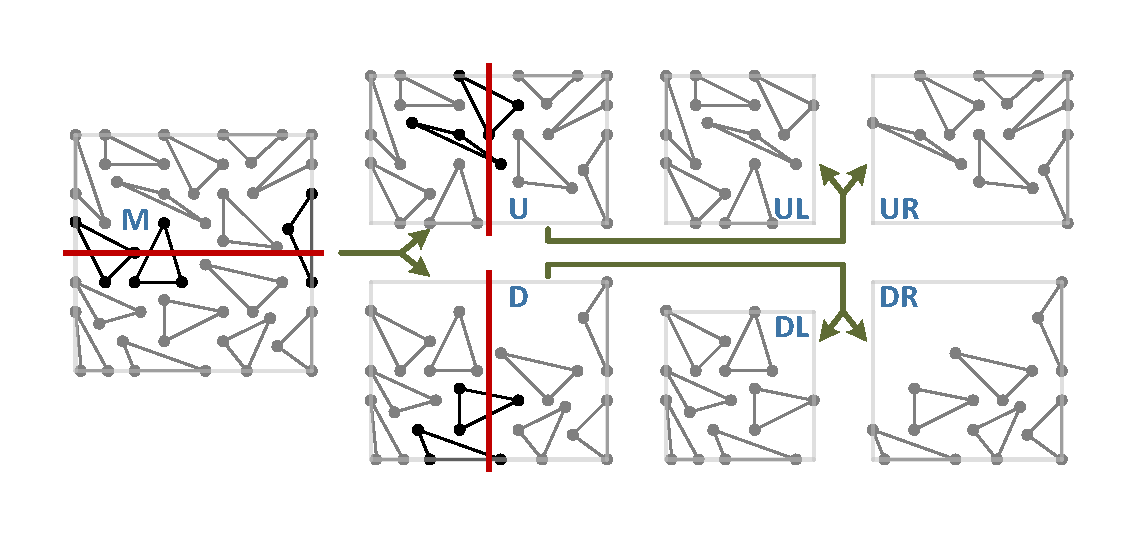
\includegraphics[width=1.0\textwidth]{pics/text_1_int/pic_box.pdf}
\singlespacing
\captionstyle{center}\caption{Схема построения дерева контейнеров.}\label{fig:text_1_int_box_tree}
\end{figure}

Для поиска потенциально пересекающихся ячеек построим дерево контейнеров всех ячеек сетки.
Корнем данного дерева будет являться контейнер всех ячеек расчетной сетки.
Рассмотрим процедуру разделения контейнера на два более мелких на примере двумерного случая, проиллюстрированного на рис.~\ref{fig:text_1_int_box_tree}.
Путь мы хотим разделить контейнер некоторого множества треугольников ($M$) по горизонтальной прямой на два множества: верхнее ($U$) и нижнее ($D$).
Тогда в верхнее множество попадут все треугольники, лежащие выше прямой, либо пересекающие ее.
Аналогично в нижнее множество попадут все треугольники, лежащие ниже прямой, либо пересекающие ее.
После выделения верхнего и нижнего множества треугольников, для каждого из них строятся свои контейнеры, которые становятся дочерними контейнерами исходного.
После этого получившиеся контейнеры можно делить дальше, используя произвольное направление разбиения ($X$, $Y$, $Z$).
В частности на рис.~\ref{fig:text_1_int_box_tree} продемонстрировано разбиение исходного контейнера по схеме $[M] \rightarrow \{[U], [D]\} \rightarrow \{\{[UL], [UR]\}, \{[DL], [DR]\}\}$.
Следует заметить, что за одну операцию контейнер можно разбивать на произвольное количество дочерних контейнеров аналогичным образом.
В качестве же направления разбиения контейнера целесообразно выбирать наиболее протяженное (вдоль которого длина контейнера имеет наибольшее значение).

Построенное дерево контейнеров позволяет существенно сократить количество проверяемых потенциальных пересечений треугольников \cite{Jung2004Int}, так как если $[M] \cap [M'] = \emptyset$, $[T]$ -- дочерний контейнер для $[M]$, а $[T']$ -- дочерний контейнер для $[M']$, то $[T] \cap [T'] = \emptyset$.

После того, как найдены все пары потенциально пересекающихся треугольников, необходимо проверить, пересекаются ли они на самом деле (см. раздел~\ref{sec:text_1_geo_prim_tri_tri}).

\subsubsection{Обработка пересекающихся треугольников}

После того, как найдены все пары пересекающихся ячеек и области их пересечения, необходимо определить стратегию их устранения.
Все ячейки расчетной сетки можно разделить на три категории.
Первая категория -- ячейки, которые не пересекаются ни с какими другими ячейками, и которые должны стать частью итоговой поверхности (будем считать, что в любой момент времени у нас есть возможность указать произвольное количество таких ячеек).
Будем такие ячейки называть статические\label{term:cell_static}.
Вторая категория -- ячейки, которые не пересекаются ни с какими другими ячейками, но которые не должны стать частью итоговой поверхности (ячейки внутренних петель самопересечения поверхности, которые должны быть удалены).
Такие ячейки будем называть скрытыми\label{term:cell_hidden}.
Третья категория -- ячейки, которые пересекаются с какими-то другими ячейками. 
Такие ячейки будем называть ячейками пересечения\label{term:cell_intersect}.

\begin{figure}[ht]
\centering
\begin{tabular}{lll}
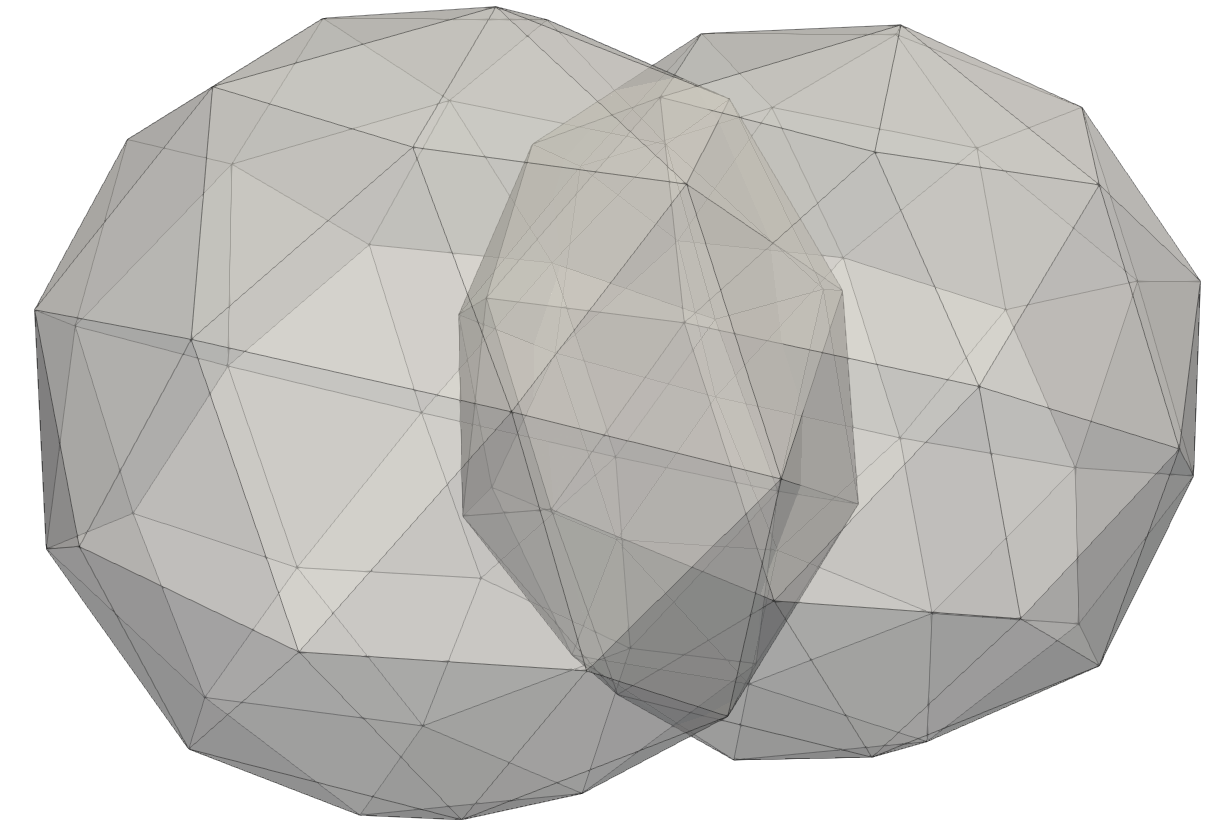
\includegraphics[width=0.3\textwidth]{./pics/text_1_int/pic_zip_01.png}
&
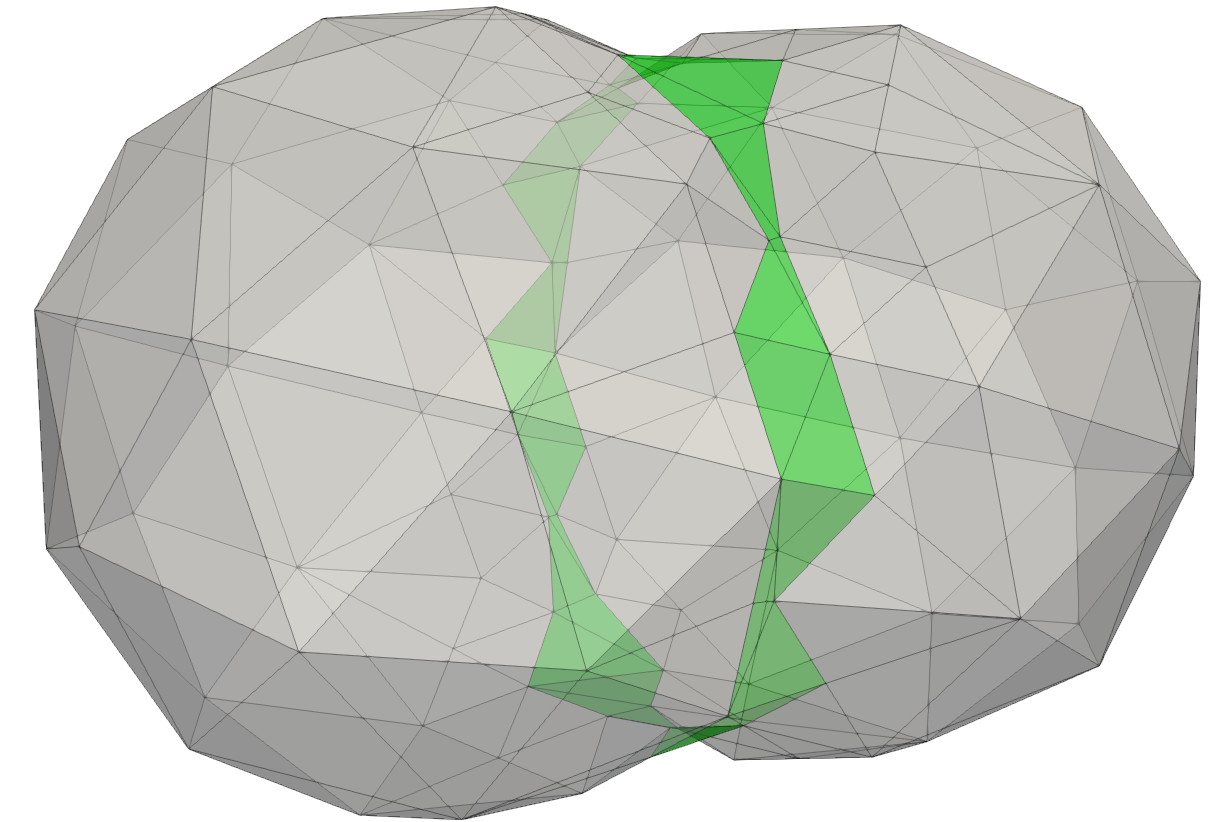
\includegraphics[width=0.3\textwidth]{./pics/text_1_int/pic_zip_09.png}
&
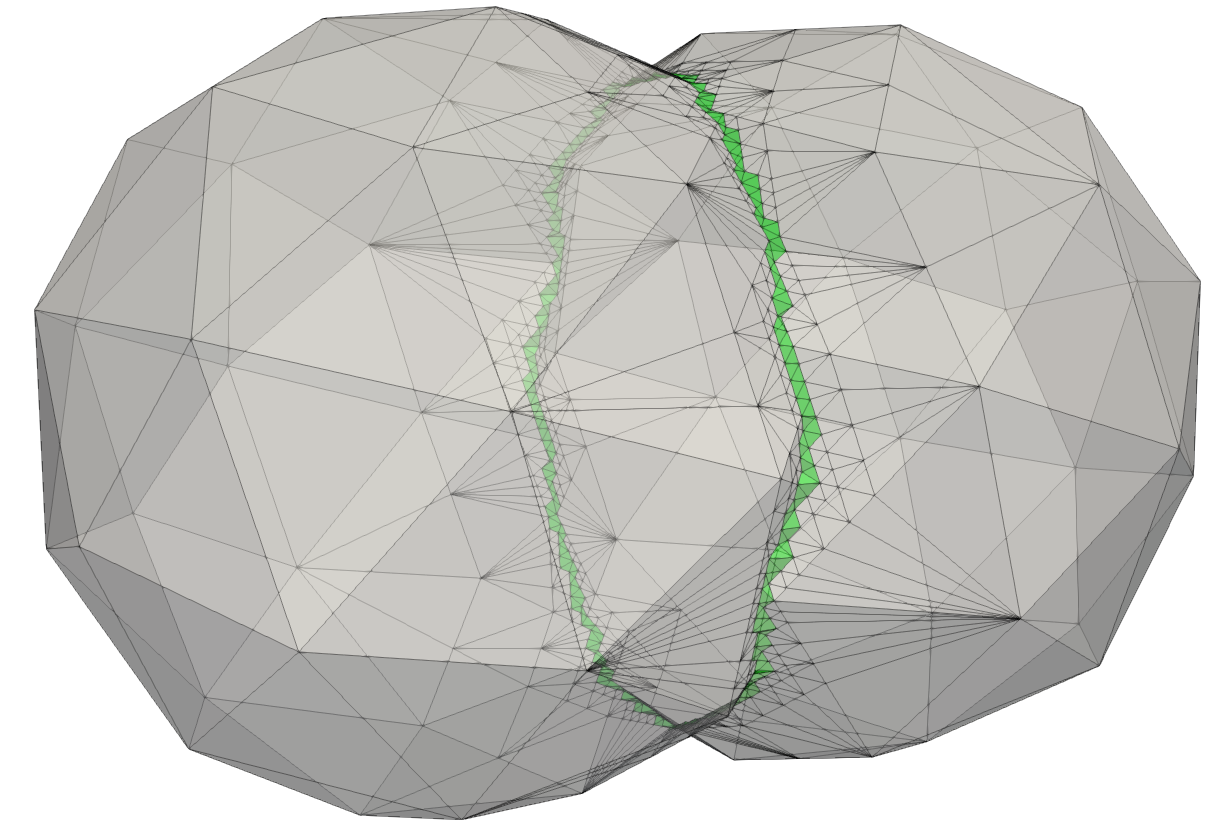
\includegraphics[width=0.3\textwidth]{./pics/text_1_int/pic_zip_15.png}
\end{tabular}
\singlespacing
\captionstyle{center}\caption{Устранение пересечений двух сфер.}
\label{fig:text_1_int_spheres}
\end{figure}

Одним из подходов к устранению самопересечений сетки является просто удаление всех ячеек пересечения.
После выполнения этой операции сетка распадается на области статических и скрытых ячеек.
При этом скрытые ячейки являются недостижимыми из статических при выполнении обхода ячеек расчетной сетки (если в процессе обхода соседними считаются только ячейки, смежные по ребру).
После удаления из сетки скрытых ячеек расчетная сетка состоит только из статических ячеек, однако требуется добавление новых ячеек для восстановления целостности сетки \cite{Charton2021Repair}.
Такой подход, который мы будем называть методом устранения самопересечений с восстановлением\label{term:method_selfint_repare}, может применяться для сравнительно простых поверхностей, но в общем случае он не гарантирует получение корректного результата.
В качестве иллюстрации такого способа устранения пересечений на рис.~\ref{fig:text_1_int_spheres} приведен пример работы для устранения пересечений расчетных сеток двух сфер (новые ячейки, появляющиеся при восстановлении сетки отмечены зеленым цветом).
На рис.~\ref{fig:text_1_int_spheres} в середине можно отметить достаточно низкое качество результирующей сетки.
Повысить качество можно с помощью дробления ячеек пересечения.
То есть после поиска всех ячеек пересечения, их необходимо раздробить на более мелкие (как показано на рис.~\ref{fig:text_1_int_cut} справа), после чего повторить процедуру удаления ячеек пересечения и скрытых ячеек и выполнить восстановление сетки.
Процесс дробления ячеек пересечения можно повторять многократно, при этом качество результирующей сетки будет повышаться, как это показано на рис.~\ref{fig:text_1_int_spheres} справа.

При другом подходе устранения самопересечений никакие ячейки из сетки не удаляются, а дробятся на более мелкие по всем точкам пересечения \cite{Skorkovska2018Int}.
Таком подход будем называть методом устранения самопересечений с дроблением\label{term:method_selfint_cut}.
В качестве примера на рис.~\ref{fig:text_1_int_tri_cut} слева показаны два треугольника, которые пересекаются по отрезку (две точки пересечения).
После выполнения дробления получаем конструкцию, показанную на рис.~\ref{fig:text_1_int_tri_cut} справа.
В общем случае точек, по которым необходимо разбивать ячейку, может быть сколь угодно много, и дробление должно выполняться с помощью выполнения триангуляции по этим точкам, причем некоторые ребра триангуляции должны быть фиксированы.

\begin{figure}[ht]
\centering
\begin{tabular}{ll}
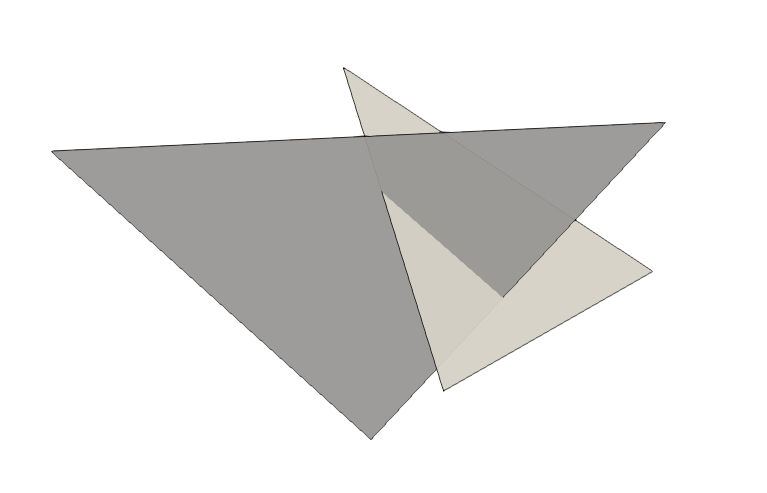
\includegraphics[width=0.35\textwidth]{./pics/text_1_int/pic_before_cut.png}
&
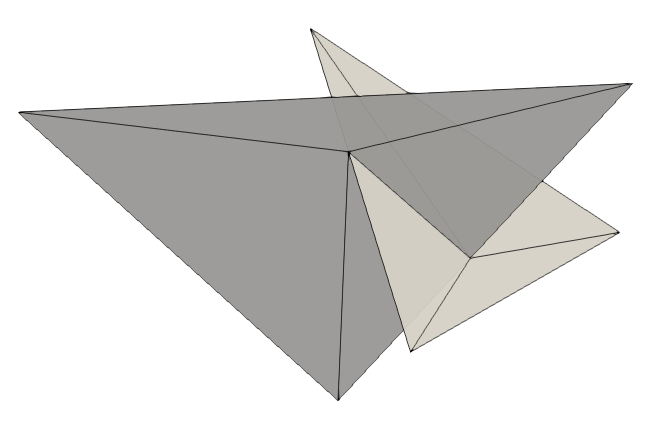
\includegraphics[width=0.35\textwidth]{./pics/text_1_int/pic_after_cut.png}
\end{tabular}
\singlespacing
\captionstyle{center}\caption{Разбиение треугольника по точкам пересечения.}
\label{fig:text_1_int_tri_cut}
\end{figure}

После дробления ячеек по точкам пересечения, между ячейками сетки могут остаться только следующие виды отношений: две ячейки не имеют общих точек, две ячейки имеют одну общую вершину, две ячейки имеют одно общее ребро.
При этом в сетке появляются ребра, имеющие более двух инцидентных ячеек.
Если наложить на исходную сетку два дополнительных условия, которые могут быть достигнуты с помощью локальных преобразований сетки, то можно добиться достаточно простой структуры сетки (такие сетки будем называть простыми\label{term:mesh_simple}).
Первым условием будем считать отсутствие в сетке совпадающих вершин.
Вторым условием будем считать то, что никакой узел сетки не находится ни в какой другой ячейке.
При выполнении этих двух дополнительных условий можно утверждать, что если ребро имеет более двух инцидентных ячеек, то это количество в точности равно 4, причем эти 4 инцидетные ячейки попарно находятся в одной плоскости.

\begin{figure}[ht]
\centering
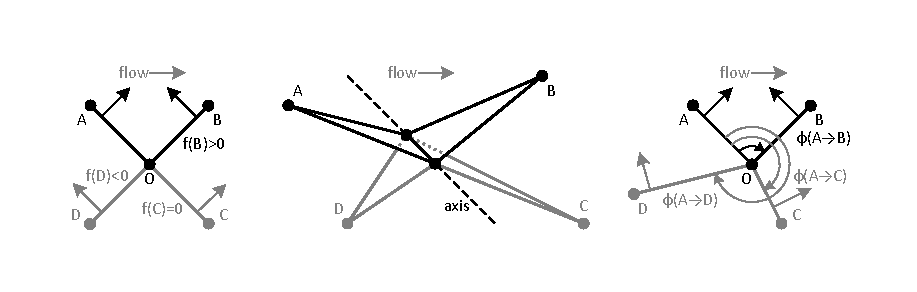
\includegraphics[width=0.9\textwidth]{pics/text_1_int/pic_walk_1.pdf}
\singlespacing
\captionstyle{center}\caption{Схема обхода результирующей поверхности.}
\label{fig:text_1_int_walk}
\end{figure}

Для получения результирующей поверхности необходимо избавиться от лишних ячеек, чтобы у каждого ребра вновь осталось ровно по 2 инцидентные ячейки.
Для этого нужно выполнить обход сетки, начиная с любой статической ячейки, считая соседними две ячейки, имеющие общее инцидентное ребро (помечаемые в процессе обхода ячейки попадут в результирующую сетку).
При движении от некоторой ячейки через ребро, имеющее более двух инцидентных ячеек, возникает вопрос выбора ячейки, которая должна войти в результирующую сетку (при этом все остальные ячейки должны быть удалены).

Рассмотрим процедуру выбора следующей ячейки обхода сетки для ребер, имеющих количество инцидентных ячеек, больше двух (рис.~\ref{fig:text_1_int_walk}, в центре).
На данном рисунке обозначено направление обхода слева направо, вслед за ячейкой, инцидентной вершине $A$, в результирующую сетку должна войти ячейка, инцидентная вершине $B$.
Рассмотрим эту процедуру для простых сеток, а также для сеток в общем виде.
Для простоты будем рассматривать задачу в проекции на плоскость, перпендикулярную ребру.

Для начала будем считать, что имеет место случай простой сетки (рис.~\ref{fig:text_1_int_walk}, слева).
Пусть уже известно, что ячейка, инцидентная вершине $A$, помечена, а ее внешняя нормаль равна $\overline{n}_A$.
Из оставшихся трех ячеек (инцидентных вершинам $B$, $C$, $D$ соответственно) необходимо выбрать только одну для продолжения обхода сетки, а остальные удалить.
Так как сетка у нас простая, то $\angle AOC = \angle BOD = \pi$, а значит $(\overline{n}_A, \overline{OB}) > 0$, $(\overline{n}_A, \overline{OC}) = 0$, $(\overline{n}_A, \overline{OD}) < 0$.
Таким образом, из всех ячеек, необходимо выбрать ту, для которой значение $(\overline{n}_A, \overline{OP})$ максимально.

Теперь рассмотрим расчетную сетку в общем виде.
В этом случае количество ячеек, инцидентных рассматриваемому ребру, может быть произвольным, больше двух, а про значение функции $(\overline{n}_A, \overline{OP})$ сказать ничего нельзя.
Для выбора следующей ячейки для обхода сетки будем поворачивать текущую ячейку вокруг рассматриваемого ребра в направлении $\vec{n}_A$ до совпадения с первой ячейкой (рис.~\ref{fig:text_1_int_walk}, справа).
Первая ячейка и должна быть выбрана в качестве следующей для продолжения обхода.
Если через $\phi(A \rightarrow P)$  обозначить угол поворота исходной ячейки в направлении $\overline{n}_A$ до ячеки, инцидентной вершине $P$, то в качестве следующей ячейки для обхода необходимо выбрать ту, для которой $\phi(A \rightarrow B)$ будет минимально.

Объединяя вместе оба рассмотренных случая, получаем критерий выбора следующей для обхода ячейки: должна быть выбрана ячейка, для которой значение показателя $f(P)$ максимально, где $f(P) = (\overline{n}_A, \overline{OP})$ для простых сеток и $f(P) = -\phi(A \rightarrow P)$ в общем случае.

\begin{figure}[ht]
\centering
\begin{tabular}{ll}
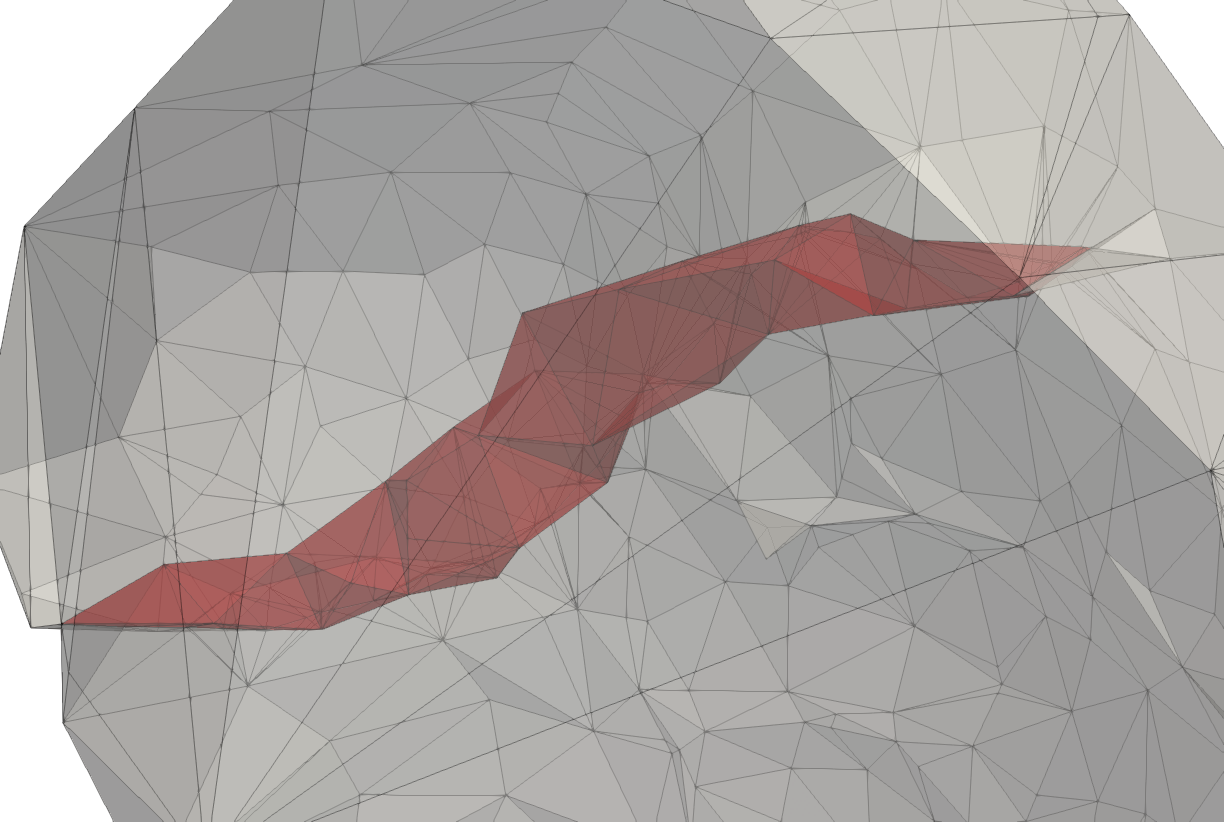
\includegraphics[width=0.45\textwidth]{./pics/text_1_int/pic_self_intersection_on.png}
&
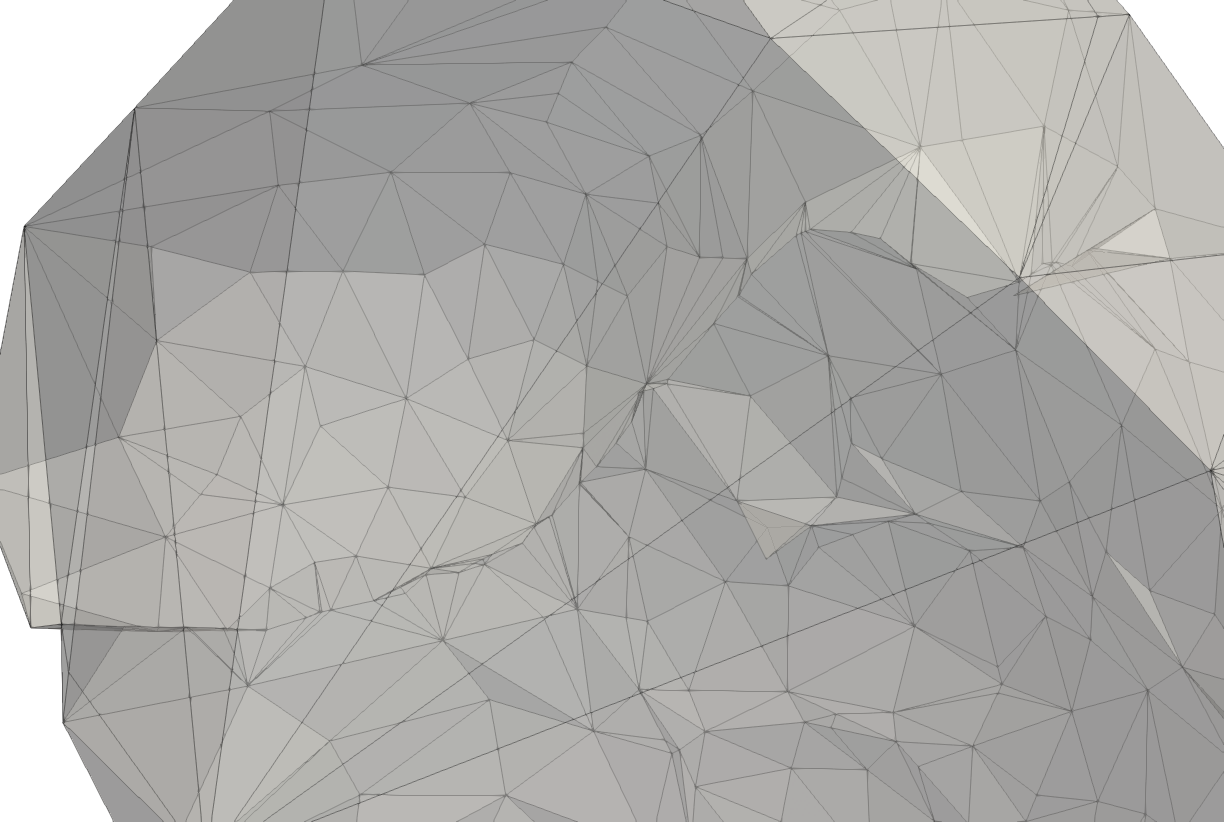
\includegraphics[width=0.45\textwidth]{./pics/text_1_int/pic_self_intersection_off.png} \\
\\
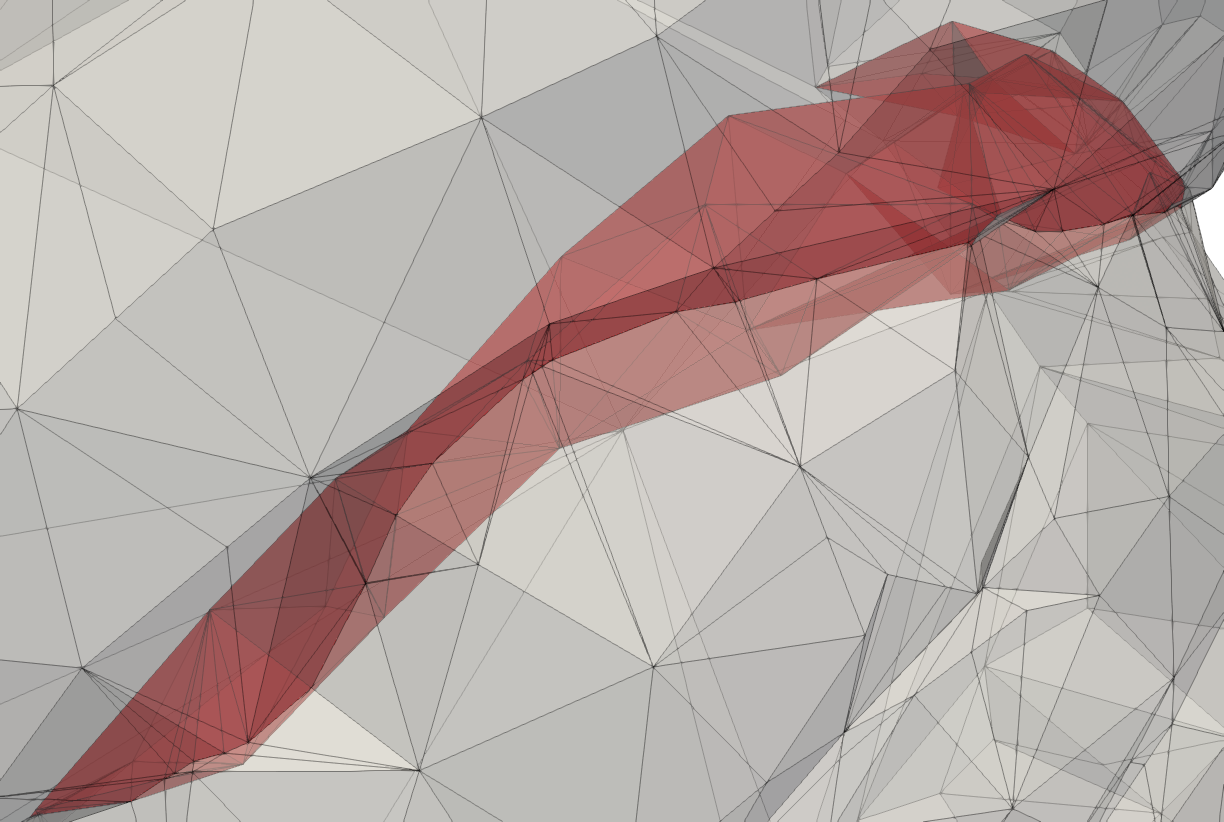
\includegraphics[width=0.45\textwidth]{./pics/text_1_int/pic_self_intersection_on_2.png}
&
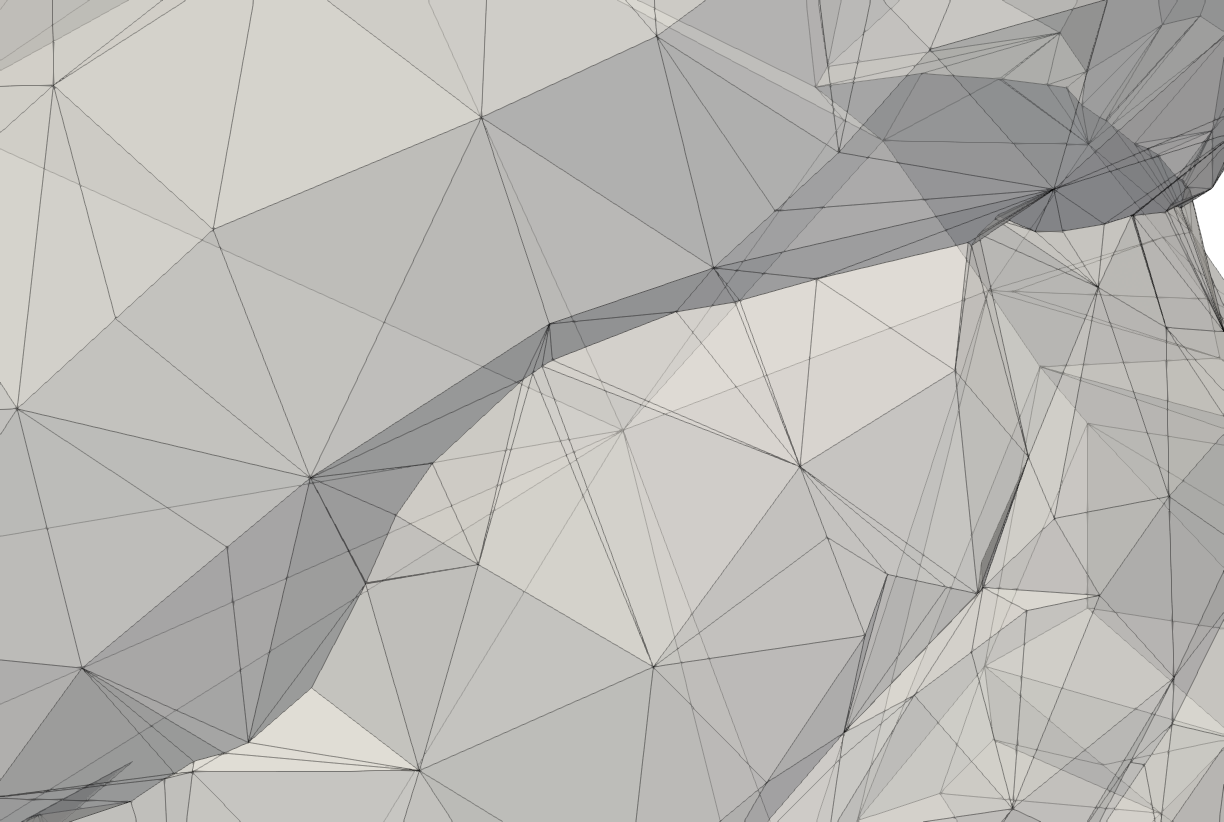
\includegraphics[width=0.45\textwidth]{./pics/text_1_int/pic_self_intersection_off_2.png}
\end{tabular}
\singlespacing
\captionstyle{center}\caption{Демонстрация удаления самопересечений.}
\label{fig:text_1_int_selfintoff2}
\end{figure}

После завершения обхода расчетной сетки все помеченные ячейки считаются ячейками целевой поверхности, а все остальные ячейки должны быть удалены.
На рисунке рис.~\ref{fig:text_1_int_selfintoff2} проиллюстрированы примеры устранения самопересечений сетки в виде скрытых петель.
После удаления скрытых ячеек целевая расчетная сетка снова становится корректной, удовлетворяет соотношениям \eqref{eqn:text_1_remesh3_arch} и может быть использована для дальнейшего моделирования ледообразования.
